\cotefile{76}
\scanpage{19}
% L1–4
On trouve que $n\longmapsto D[n]$ devient un ens quasi-simplicial, i.e un \unsure{contrafoncteur} sur la catégorie $\unsure{\mathbb{\Delta}|\Delta}$ des ens finis non vides de la forme $\Delta_n=[0,n]_{\mathbb N}$, avec comme
% L5–7
morphismes les appl. \uline{injectives}. Cet ens quasi-simplicial satisfait la condition que
% L8
$\forall n,m\in\mathbb N$ avec $n<m$, et $d_m\in D[m]$, l'application
% L9–10
\[
\begin{aligned}
\mathrm{Hom}_{\mathbb{\Delta}}(\Delta_n,\Delta_m)&\longrightarrow D_n\\
u&\longmapsto u^*(d_m)
\end{aligned}\tag*{\unsure{(*)}}
\]
% L11–12
est injective, qui signifie aussi que la catégorie
% L13
\[
\widehat{\mathbb{\Delta}}/D[\,]
\]
% L14
est ordonnée (\unsure{ou mieux|ou même|ou au moins|i.e. équivalente}, préordonnée).

% L15–17
L'ens ordonné $D$ se reconstitue en \deleted{\unsure{fon|fonction}} \unsure{termes|fonction} du $D[\,]$, comme l'ens ordonné \deleted{\unsure{que}} défini par la dite catégorie ordonnée. \deleted{\unsure{Inversement}}, \inserted{\unsure{On trouve}}
% L18
\deleted{la donnée de l'ens \unsure{f}}
% L19–22
\diagram{\begin{tikzcd}[ampersand replacement=\&,column sep=small]
\begin{gathered}\text{géométrie des drapeaux }D\\
\text{avec syst. d'ordres }\text{\inserted{totaux}}\ \unsure{\text{coh.}|\text{etc.}}\ \text{sur}\\
\text{les simplexes des } \unsure{\mathscr D|\Phi}\ (\text{ens des}\\
\text{él. minimaux de }D)\end{gathered}
\arrow[r,leftrightarrow] \&
\begin{gathered}\text{ens quasi-}\\\text{simpliciaux}\\
\text{satisfaisant la}\\\text{condition }(*)\text{.}\end{gathered}
\end{tikzcd}}
% archive sheet number: 18
\scanpage{20}
% L1–3
Soit $D$ une géométrie de drapeaux quasi-simpliciale
\[
\deleted{D:\bigl(\unsure{A}\big/\underline{P_f}^{*}(\mathbb N)\bigr)^{\circ}\longrightarrow(\mathrm{Ens})}
\]
\deleted{une \uline{\textquotedblleft géométrie de drapeaux avec fonction-dimension\textquotedblright},}
% L4–5
[i.e avec \unsure{$D$\,:|$D$\,;|$D$} un syst. d'ordres totaux compatibles, sur les simplexes de $\unsure{\mathscr D|\mathscr F|\Phi}=D_0$ (ens des él. minimaux de $\mathscr D$)]
% L6–7
d'où
\[
X=|D|
\]
% L8–10
espace topologique, muni de parties fermées (en fait, des simplexes)
\[
X(d)\qquad d\in D
\]
% L11–13
définissant une \deleted{\unsure{structure}} \inserted{stratification} \unsure{cônique|conique|canonique} de $X$ par des simplexes (les $X^{\circ}(d)=X(d)\setminus\bigcup_{d'<d}X(d')$ \unsure{font|forment} une partition de $X$ par des simplexes ouverts...).

% L14
Pour tout $F\in\mathscr D$, soit
% L15–17
\[
\left\{\begin{aligned}
|F|&=\bigcup_{\substack{d\in D_{\unsure{*|\bullet}}\\
\text{t.q. }\deleted{\unsure{\sup I_d\in F}}\\ \sup(I_d)=F}}X(d)\\
|F|^{\circ}&=\bigcup_{\text{idem}}X(d)^{\circ}
\end{aligned}\right.
\]
% L15–17 right
\margin{$\displaystyle\bigcup_{F'<F}|F'|^{\circ}$\\
$\parallel$\\
$\displaystyle |F|-|F|^{\circ}\mathrel{\overset{?}{=}}\bigcup_{\substack{\deleted{\unsure{d\in D_*}}\\F'<F}}|F'|$\\
$\parallel$\\
$\displaystyle\bigcup_{\substack{d\in D_*\\\sup I_d<F}}X(d)$}
% L18–20
\margin{?}
Quand peut-on dire que la famille \inserted{des} $(|F|)_{F\in\mathscr D}$
\deleted{\unsure{forme}} \inserted{est celle des cellules fermées} d'une \uline{stratification} de $X$, dont les cellules ouvertes sont les $|F|^{\circ}$ ?

% L21
\margin{En fait}
\deleted{a) $|F|$ fermés $\bigcup_{F\in\mathscr D}|F|=\bigcup_{d\in D_*}X(d)=X$}
% L22–24
a) Les $|F|^{\circ}$ \inserted{loc. fermés ??} font partition de $X$
[\uline{NB} $|F|^{\circ}\ni\deleted{\unsure{\varnothing}}\unsure{\mathrm{V}|X}(F)$
\inserted{\unsure{espace ambiant|espaces ambiants|le point représentant|les sommets maximaux}} donc $|F|^{\circ}\ne\varnothing$]

% L25
b) $|F|=\overline{|F|^{\circ}}$ (car $X(d)=\overline{X(d)^{\circ}}$) \margin{réunion de \textquotedblleft cellules ouvertes\textquotedblright\ \unsure{...}}

% L26
\deleted{c) $|F|^{\circ}=|F|\setminus\bigcup_{\unsure{G< F}}\bigcup_{\substack{d\in D_*\\\sup(I_d)=F}}(X(d)$}
% archive sheet number: 19
\scanpage{21}
% L1–2
Soit $\unsure{\mathbb{\Delta}|\Delta}$ la catégorie des ens finis $\mathrm{tot}^{\mathrm t}$ ordonnés \inserted{non vides}, avec comme morphismes les applications \uline{strictement} croissantes.
% L3
Soit
\[
\unsure{\mathbb D|D}_{*}\in\mathrm{Ob}\widehat{\mathbb{\Delta}}
\qquad \mathbb D_*:\mathbb{\Delta}^{\circ}\longrightarrow(\mathrm{Ens})
\]
% L4–7
donc $\mathbb D_*$ définit une catégorie fibrée à fibres discrètes sur $\mathbb{\Delta}$, à quelle condition celle-ci est-elle ordonnée \inserted{(ou préordonnée, celà revient au $=$)} ? Posons $\Delta_n=[0,n]\in\mathrm{Ob}\,\mathbb{\Delta}$, $\mathbb D_n=\mathbb D_*(\Delta_n)$, la condition est celle-ci
% L8–10
\textcircled{1} $\forall n,m\in\mathbb N$, avec $n<m$, et $d_m\in\mathbb D_m$, l'application
\[
\mathrm{Hom}_{\mathbb{\Delta}}(\Delta_n,\Delta_m)\longrightarrow\mathbb D_n
\qquad u\longmapsto u^*(d_m)
\]
est injective.

% L11–13
Ceci posé, on a donc un ens ordonné $\mathbb D_*=\coprod_{m\in\mathbb N}D_m$ et un foncteur fibrant
\[
\underline{D}_*\longrightarrow\mathbb{\Delta}
\]
% L14–18
Considérons la réalisation topologique \inserted{$|D_*|$} de $D_*$, donc $\forall d\in D_*=\mathrm{Ob}\,\underline D$, on a une partie \inserted{fermée} $|d|\subset|D_*|$, l'application $d\longmapsto|d|$ de
\[
D_*\longrightarrow\mathscr P_f(|D_*|)
\]
étant injective et préservant la relation d'ordre.
% L19–21
Considérons \inserted{pour $d_m\in\mathbb D_m$ \deleted{\unsure{$m$}}} l'ens $D_d=\{\delta\in D\mid\delta\leq d\}$, on trouve qu'il est $\mathrm{can}^{\mathrm t}$ isom (comme ens. ordonné) à $\mathscr P^*(\Delta_m)$ ($\mathscr P^*$ désigne l'ens des parties $\ne\varnothing$).
% L22–24
Donc $|d|$ est canoniquement isomorphe au simplexe type $|\Delta_m|$. Ainsi on trouve
\[
|D_*|=\varinjlim_{d\in D_*}|d|=\varinjlim_{d\in D_*}|\Delta_m|
=\varinjlim_{\Delta\in\mathbb{\Delta}/D}|\Delta|
\]
% archive sheet number: 20
\scanpage{22}
% L1–2
donc $|D_{*}|$ est aussi la réalisation topologique de l'ens quasi-simplicial $D_*$
% L3–5
L'ens ordonné $D_*$ a la propriété suivante
\textcircled{a} $\forall d\in D_*$, l'ens \inserted{ord} $D_*(d)=\{\delta\in D_*\mid\delta\leq d\}$ est isomorphe à un $\mathscr P^*(I_d)$, pour $I_d$ ens fini
% L6–9
(déterminé à isom can près comme l'ens des él. minimaux de $D_*(d)$, ou encore l'ens des éléments minimaux de $D_*$ -- \deleted{\unsure{qui}} i.e. des él. de $D_0$ -- majorés par $d$)

% L10–14
Mais comment exprimer l'ordre total des $I_d$ \inserted{$(d\in D_*)$} en termes d'une structure suppl. sur l'ens ordonné $D_*$ ? [Souvent elle sera induite par une structure d'ordre (pas total) sur $D_0$, ens des él. minimaux de $D_*$.]
% L15–18
La donnée de cet ordre total, avec la condition que pour $d'<d$, l'ordre total de $I_{d'}$ est induit par celui de $I_d$, \uline{équivaut} à la donnée de l'ens quasi-simplicial $\unsure{\mathbb D|D}_*$. On va examiner des
% L19–21
\margin{$\vert\,\vert\,\vert$}conditions \inserted{sur $D_*$} moyennant les quelles les ordres totaux des $I_d$ $(d\in D_*)$ sont bien induits par un ordre unique sur $D_0$.

% L22–23
Considérons
\diagram{\begin{tikzcd}[ampersand replacement=\&,column sep=large]
\mathbb D_0 \& D_1\arrow[l,shift right=1.5,"\partial_0"']\arrow[l,shift left=1.5,"\partial_1"] \&
D_2\arrow[l,shift right=3,"\partial_0"']\arrow[l,"\partial_1" description]\arrow[l,shift left=3,"\partial_2"]
\end{tikzcd}}
% L24
Considérons Sur $\unsure{D|D_0|\underline D}$ la relation
% archive sheet number: 21
\scanpage{23}
% L1
\[
x_0\precy_0\mathrel{\overset{\text{déf}}{\Longleftrightarrow}}
\unsure{!}\,\exists z_1\in D_1\quad\text{t.q.}\quad x_0=\delta_0(z_1),y_0=\delta_1(z_1)
\]
% L1–4 left
% slanted
\margin{\deleted{\unsure{Bref, faut} introduire une \textquotedblleft fonction dimension\textquotedblright\ $\delta$, et exiger (pour $x_0<y_0$) que $\delta(x_0)<\delta(y_0)$, pour rendre la relation écrite \unsure{non-symétrique|anti-symétrique} !}}
% L2
La condition \uuline{est} $x_0<y_0$ dans le \textquotedblleft simplexe\textquotedblright\ $\unsure{\{x_0,y_0\}}$
\deleted{\unsure{C'est la}}
% L3–4
\deleted{A-t-on transitivité pour cette relation ? \unsure{Soit}}
\textcircled{$2^{\circ}$} La relation $\prec$ \deleted{\unsure{est dans|est bien}} sur $D_0$ est transitive.
\margin{?}
Ceci si on suppose satisfaite la condition suivante
% L5–7
\deleted{\textcircled{\unsure{2$'$}}}\inserted{\textcircled{2 bis}} L'application canonique
\[
D_2\xrightarrow{(\delta_2,\delta_0)}(D_1,\delta_1)\mathbin{\times}_{D_0}(D_1,\delta_0)
\]
est surjective,

% L8–13
Car si $x_0\prec y_0$ et $y_0\prec z_0$, i.e.
\[
x_0=\delta_0(z_1),y_0=\delta_1(z_1),\deleted{\unsure{x_0|y_0}}y_0=\delta_0(z'_1),z_0=\delta_1(z'_1),
\]
$\exists u_2\in D_2$ avec $z_1=\delta_2(u_2),z'_1=\delta_0(u_2)$, posons alors $z''_1=\delta_1(u_2)$, on a
\[
\begin{aligned}
\delta_0(z''_1)&=\delta_0\delta_1(u_2)=\delta_0\delta_2u_2\\
&=\delta_0(z_1)=x_0,\quad\delta_1(z''_1)=\delta_1\delta_1(u_2)=\delta_1\delta_0(u_2)=\delta_1(z'_1)=z_0,
\end{aligned}
\]
donc $x_0\prec z_0$, cqfd. \deleted{Je dis que la relation de \unsure{préor|préordre}}
% L14–15
Ainsi, posant
\[
x_0\unsure{\preceq|\leq|\preccurlyeq} y_0\mathrel{\overset{\text{déf}}{\Longleftrightarrow}}x_0=y_0\ \text{ou}\ x_0\prec y_0
\]
% L16–17
on trouve une relation de préordre dans $D_0$, \inserted{moyennant \textcircled{$2^{\circ}$}.}
\inserted{C'est une relation d'ordre, car $x_0\prec y_0$ et $y_0\prec x_0$ sont impossibles}
% L17–20 left
% slanted
\margin{sinon $x_0\prec x_0$ i.e. $\exists z_1$ avec $\delta_0(z_1)=\unsure{\delta_0|\delta_1}(z_1)=x_0$, impossible par \textcircled{1}. Cet ordre sur $D_0$ satisfait la condition \textcircled{b} Si $x_0\prec y_0$, $(x,y\in D_0)$ \deleted{\unsure{$\delta$|$\exists$}} $\exists z\in D_*$ tel que $x_0<z,y_0<z$}
% L18–21
Ceci \deleted{\unsure{dit}} posé, si $d\in D_*$, on voit que la relation d'ordre sur $I_d=\{x\in D_0\mid x<d\}$ est induite par la relation précédente. En effet, si $x,y\in D_0$, $x,y<d$ si on a
% L22–25
$x<y$ dans \deleted{\unsure{$\Delta_d,I$}} $I_d$, \unsure{alors} on a $x\prec y$, i.e. \inserted{l'inclusion} $I_d\hookrightarrow D_0$ est strictement croissante, d'où on déduit facilement \deleted{que} (l'ordre de $I_d$ étant total \inserted{et $D_0$ étant ordonné (\unsure{non pas seulement préord.!|non pas que préord.|voir paragraphe précédent})}) que l'ordre de $I_d$ est induit par celui de $D_0$.
% archive sheet number: 22
\scanpage{24}
% L1–4
Inversement, soit $D_{*}$ un ens. ordonné satisfaisant \textcircled{a} ci-dessus. Donnons nous sur $D_0$ (ens des él. minimaux de $D_*$) une structure d'ordre (pas seulement de préordre) \inserted{notée $x\unsure{\preceq|\leq|\preccurlyeq}y$}, \deleted{\unsure{traduisant|induisant} \unsure{ce que}}
% L5–8
\inserted{satisfaisant \textcircled{b} ci-dessus et de plus}
\deleted{\unsure{signifiant que|vérifiant que}} \inserted{\textcircled{c} Elle \deleted{\unsure{sur}} induit sur} les $I_d$ \deleted{$(d\in D_*)$} $=\{x\in D_0\mid x\leq d\}$ un ordre total. \deleted{qui} \inserted{Ce dernier} est évidemment fonctoriel \deleted{\unsure{ses ordonnés|pour ordonné} (pour l'ordre induit par}
% L9–12
en $d$, de sorte que $D_*$ définit un foncteur \unsure{croissant|covariant} $\underline{D_*}\longrightarrow\unsure{\mathbb{\Delta}|\Delta}$, qui est \uline{fibrant}, à fibres discrètes -- donc associé à un foncteur $D_*:\mathbb{\Delta}^{\circ}\longrightarrow(\mathrm{Ens})$, et $D_0=D_*(\Delta_{\unsure{n|0}})$
% L13–15
(plus gén. $D_n=D_*(\Delta_n)$ est l'ens des $d\in D_*$ tels que $\mathrm{Card}(I_d)=n+1$ \unsure{$\}$}, i.e. $I_d\simeq\Delta_n$), et $D_*$ satisfait évidemment \textcircled{1}.

% L16–23 left
\diagram{\begin{tikzcd}[ampersand replacement=\&,row sep=large]
\begin{gathered}\text{Ens. quasi-simpliciaux }\text{\inserted{$D_*$}}\text{ satisfaisant}\\
\text{\textcircled{1} et \textcircled{2}}\end{gathered}\arrow[d,shift right=5]\\
\begin{gathered}\text{Ens ordonnés }\text{\inserted{$D_*$}}\text{ satisfaisant \textcircled{a} et}\\
\text{munis d'une relation d'ordre}\\
\text{sur }D_0=\text{ ens des él minimaux}\\
\text{de }D_*\text{, satisfaisant les conditions}\\
\text{\textcircled{b} et \textcircled{c}}\end{gathered}\arrow[u,shift right=5]
\end{tikzcd}}
% L16–20 right
Soient alors $x_0,y_0\in D_0$ tels que $x_0\prec_{*}y_0$ i.e. $\exists z_1\in\unsure{\mathbb D|D}_1$, $x_0=\delta_0(z_1),y_0=\delta_1(z_1)$ avec $z_1\in D_1$. Donc $I_{z_1}=\{x_0,y_0\}$, et par définition de $\delta_0,\delta_1$, $x_0$ est
% L21–24 right
le $\mathrm{1}^{\mathrm{er}}$ él de $I_{z_1}$ pour l'ordre \inserted{(total)} induit par $D_0$ $y_0$ le deuxième, i.e. on a $x_0\prec y_0$. Inversement,
% L25–27
supposons $x_0\prec y_0$, \deleted{donc} $\exists\unsure{z|d}\in D_*$ tel que $x_0<z,y_0<z$ -- on aura $z\in D_n$ avec $n\geq1$, $x_0,y_0$ él. distincts de $I_z$, \deleted{donc} on a $x_0\prec y_0$ pour
% archive sheet number: 23
\scanpage{25}
% L1–3
l'ordre induit par $(D_0,\prec)$, \deleted{ce qui} correspond à une \deleted{\unsure{application}} \inserted{morphisme} $\sigma:\unsure{\mathbb{\Delta}|\Delta}_1\unsure{\mathrel{-}|\longrightarrow}\mathbb{\Delta}_n$, \unsure{tel|telle} que, posant $z_1=\sigma^*(u)$, on ait $x_0=\delta_0(z_1),y_0=\delta_0(z_1)$, i.e. on
% L4–7
a $x_0\prec_*y_0$. Ainsi l'ordre $\prec$ donné à l'avance sur $D_0$ (satisfaisant \textcircled{b}) se récupère à partir de la donnée quasi-simpliciale $D_*$ qu'il définit, comme étant $\prec_*$.

% L8–11
\uline{Rmq} Supposons donné l'ens ordonné $D_*$, \inserted{satisfaisant \textcircled{a},} et supposons qu'il existe un ordre $\omega$ sur $D_0$ satisfaisant \textcircled{b}. Alors l'ordre opposé $\omega^{\circ}$ satisfait également \textcircled{b}, mais donne lieu bien
% L12–14
sûr à une autre loi quasi-simpliciale sur la famille des $D_n=\{d\in D_*\mid\mathrm{Card}\,I_d=n+1\}$ (sauf si $D_1=0$ i.e. l'ordre de $D_*$ est discret).
% L15–17
Néanmoins, comme les \inserted{réalisations top. des} deux ens. quasi-simpliciaux obtenus sont \unsure{can.} homéom. à la réalisation top \inserted{$|D_*|$} de l'ens ordonné $D_*$,
% L18–20
(qui, elle, ne dépend pas du choix d'un ordre sur $D_0$) on trouve \deleted{que les 2} \inserted{un homéom. can} \deleted{ens quasi-simpliciaux}
\[
|D_*^{\omega}|\simeq|D_*^{\omega'}|
\]
% archive sheet number: 24
\scanpage{26}
% L1–4
\uline{Ex 1} Soit $\unsure{\mathfrak X|\mathscr X}$ un ens ordonné. Soit $D_*$ l'ens des parties finies de $\mathfrak X$, $\mathrm{tot}^{\mathrm t}$ ordonnées par l'ordre \unsure{induit|induite} (\textquotedblleft drapeaux de $\mathfrak X$\textquotedblright)\,; on ordonne $D_*$ par inclusion.
% L5–7
Alors $D_0$ (en tant qu'ens) \deleted{\unsure{est}} s'identifie à $\mathfrak X$, il est \deleted{\unsure{ordon|ordonné}} donc muni d'une relation d'ordre, et \textcircled{a} et \textcircled{b} sont évidemment satisfaites.
% L8–10
D'où un ens. quasi-simplicial $D_*$, et on a des homéom. can
\[
|D_*|\simeq|\unsure{\mathscr D|D}_*|\simeq|\mathfrak X|
\]
% L11–13
En fait, les $(D_*,\prec)$ obtenus sont ceux pour les quels on a, en plus de \textcircled{a}, \textcircled{b}, \inserted{\textcircled{c}} la condition
\[
\text{\textcircled{d}}\quad\forall d\in D_*,\ \text{on a}\quad d=\mathrm{Sup}(I_d)
\]
% L14–15
i.e. l'ens ordonné $D_*$ est l'ens des simplexes \inserted{non vides} d'une \uline{maquette simpliciale}, \deleted{$D_*$ sur \unsure{où l'ens quasi-simplicial des}}
% L16–20
Donc il faut prendre les maquettes simpliciales avec une structure d'ordre sur l'ens $\mathfrak X=D_0$ des sommets, induisant un ordre total sur chaque simplexe, et \deleted{\unsure{tel que les|tel que}} \inserted{(parmi les parties finies non vides)} sur les simplexes seulement\ldots
% L21–24
[Notons aussi que \deleted{moyennant \textcircled{a} et \textcircled{b} équivaut à \unsure{c}} \inserted{\textcircled{a} $+$ \textcircled{d} (i.e. $D_*$ correspond à} maquette simpliciale) équivaut à \textcircled{a$'$} $+$ \deleted{\unsure{\textcircled{c}}} \textcircled{d}, avec
% L24
\textcircled{a$'$} Dans $D_*$ les sup \inserted{(finis)} majorés existent\ldots\ ]
% archive sheet number: 25
\scanpage{27}
% L1–4
\uline{Ex 2} Soit $G$ un gpe, et soit $(\sigma_i)_{0\leq i\leq n}$ un système d'éléments de $G$, tels que $\sigma_i,\sigma_{j\unsure{\mathrm{en}|a}}$ commutent pour \deleted{$i<j$} $n\geq j\geq i+2\geq i\geq0$. \deleted{\unsure{On en} \unsure{forme} \unsure{Ainsi} $G$\unsure{-ens, et|roupes, et}}
% L5–7
pour tte partie finie $H$ de $\Delta_n=[0,n]$, soit \deleted{\unsure{$R_H$}\unsure{ pose }\unsure{$D$}} $N_H=$ ss-gpe de $G$ engendré par $\{\sigma_i\mid i\in\Delta_n\setminus H\}$. Donc $H\subset H'\Rightarrow N_{H'}\subset N_H$.

% L8–10
Soit $X$ un $G$-ens et soit
\[
\unsure{\mathbb D|D}(H)=X/N_H\qquad\text{(drapeaux de type }H\text{)}
\]
donc $H\subset H'\Longrightarrow\inserted{i_{H,H'}^*:}D(H')\longrightarrow D(H)$,
% L11–12
$H\longmapsto D(H)$ foncteur contravariant
\[
\underline{\mathscr P(\Delta_n)}^{\circ}\longrightarrow(\mathrm{Ens})
\]
% L13
Soit
\[
D_*=\coprod_{H\in\mathscr P(\Delta_n)}D(H)
\]
% L14–17
relation d'ordre : $d\in D(H), d'\in D(H')$,
\[
d\leq d'\mathrel{\overset{\text{déf}}{\Longleftrightarrow}}H\subset H'\ \text{et}\ d=i_{H,H'}^*(d').
\]
Ceci dit, $D_*$ satisfait la condition \textcircled{a} : si $d\in D_*$ $D_*(d)\simeq\mathscr P(I_d)$ (où $I_d\simeq H$ si $d\in D(H)$).

% L18–20
Les él. minimaux sont ceux de
\[
D_0=\coprod_{0\leq i\leq n}\underbrace{D(\{i\})}_{X/(\sigma_0\mathbin{-}\widehat{\sigma_i}\mathbin{--}\sigma_n)}.
\]
% L21–22
On va introduire sur $D_0$ une relation d'ordre (pour l'instant on n'a pas utilisé la structure d'ordre total
% archive sheet number: 26
\scanpage{28}
% L1–3
sur l'ens d'indices $\Delta_n$ pour les $\sigma_i\in G$] Si \deleted{\unsure{$z$}} $x_i\in D(\{i\}),y_j\in D(\{j\})$, on pose $x_i\unsure{\prec|<}y_j$ ssi $i<j$ et $\exists z\in D_*$ tel que \deleted{\unsure{$z$}} $x_i,y_j\leq z$.
% L4–5
\deleted{Cette relation d'ordre satisfait \textcircled{b} \inserted{(par définition)} et \textcircled{c} (par définition aussi)}
% L6–8
Cette relation est-elle transitive ? Supposons $i<j<k$, $x_i\in D(\{i\}),y_j\in D(\{j\}),z_k\in D(\{k\})$, \deleted{\unsure{$x_i$}} $x_i,y_j$ viennent de $u_{ij}\in D(\{i,j\})$, $y_j,z_k$ viennent
% L9–10
de $v_{jk}\in D(\{\deleted{\unsure{i}}j,k\}.$ Donc $(u_{ij},v_{jk})$ est un élément de
\[
D(\{i,j\})\mathbin{\times}_{D(\{j\})}D(\{j,k\})
\]
% L11–14
on serait content qu'il provienne d'un \unsure{élement|élmt|élément} $w_{ijk}\in D(\{i,j,k)\}$, car il \unsure{devrais|devrait|alors|dernier} définirait un élément \deleted{\unsure{$u$}} $\unsure{\chi|\gamma|x}_{ik}\in D(\{i,k\})$ \deleted{dont} se restreignant suivant $x_i$ et $\unsure{y_k|z_k}$. Donc
% L15
on veut
\[
D(\{i,j,k\})\xrightarrow{\text{\textcircled{épi}}}D(\{i,j\})\mathbin{\times}_{D(\{j\})}D(\{j,k\})
\]
% L16
Or je dis plus généralement qu'on a

% L17–21
\uline{Lemme} Soient $H,H'\subset\Delta_n$ tels que $H\cap H'\ne\varnothing$ et $H\cap H'$ soit un segment final de l'ens tot. ordonné $H$, un segment initial de l'ens tot ordonné $H'$. Considérons l'appl. canonique
% L22
\[
D(H\cup H')\xrightarrow{\deleted{\unsure{\sim}}}D(H)\mathbin{\times}_{\substack{\deleted{\unsure{D(H)\cap D(H')}}\\ D(H\cap H')}}D(H')
\]
% L23
Celle-ci est \uline{surjective}.
% archive sheet number: 27
\scanpage{29}
% L1–3
\uline{Dém} Soit \inserted{pour $K\subset\Delta_n$,} $G_K=$ ss-gpe de $G$ engendré par $\{\sigma_i\mid i\in K\}$. Soit \deleted{$K=\complement_{\inserted{\Delta_n}}H,\ K'=\complement H'$} $K=\Delta_n\setminus H,\ K'=\Delta_n\setminus H'$, donc $K\cup K'=\Delta_n-H\cap H'$, la \deleted{diagramme} \inserted{flèche} envisagée est
% L4–5
\diagram{\begin{tikzcd}[ampersand replacement=\&]
X/G_{K\cap K'}\arrow[r,"p"] \& X/G_K\mathbin{\times}_{X/G_{K\cup K'}}X/G_{K'}\\
X\arrow[u]\arrow[ur,"p'"] \&
\end{tikzcd}}
% L6–8
Il suffit de prouver que $p'$ est surjectif. Je dis que l'on a
\[
G_{K\cup K'}=G_K\cdot G_{K'}
\]
(d'où \deleted{\unsure{l'énoncé|l'assertion}} le résultat s'ensuit aussitôt).
% L9–11
Or \deleted{\unsure{soit}} \inserted{soit} $i$ le dernier él. \deleted{de $K$}, \inserted{de $H$ \deleted{\unsure{donc}} de $H\cap H'$} \deleted{\unsure{Il vient}} $i\in H\cap H'$ \deleted{donc $K_0=K\cap[0,i-1]\subsetK'$} $i\notin K\cup K'$, donc
% L12 left
\margin{OPS $H\cap H'\ne H,H'$}
% L12–13
\[
\begin{aligned}
K\cup K'&=(K\cup K')\cap\underbrace{\complement\{i\}}_{[0,i-1]\amalg[i+1,n]}\\
&=\overbrace{(K\cup K')\cap[0,i-1]}^{K'_0}\\
&\quad\amalg\underbrace{(K\cup K')\cap[i+1,n]}_{K_0}
\end{aligned}
\]
% L14–15
Le dernier sommande est $\deleted{\unsure{\subset}}\subset K$ car $[i+1,n]\subset K$, le premier est $\subset K'$, car pour les $j\leq i-1$,
% L16–17 left
\figure{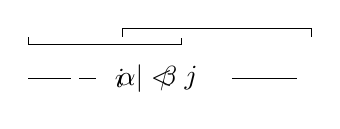
\begin{tikzpicture}[x=.75cm,y=.47cm]
\draw (0,1.1)--(0,0.9)--(2.6,.9)--(2.6,1.08);
\draw (1.6,1.12)--(1.6,1.35)--(4.8,1.35)--(4.8,1.12);
\draw (0,0)--(.72,0) (.86,0)--(1.14,0) (3.45,0)--(4.55,0);
\node at (1.55,0){$i$};\node at (1.98,0){$\unsure{\alpha|<}$};
\node at (2.38,0){$\beta$};\node at (2.76,0){$j$};
\end{tikzpicture}}
% slanted
\margin{On a utilisé a) le dernier él. de $H$ est dans $H'$ b) $H\cap H'$ est un segment initial de $H'$}
% L16–20
\deleted{\unsure{ou bien} $j\in$} Si $j\notin H\cap H'$ (i-e. $j\in K\cup K'$) \deleted{ou bien} \inserted{on a} $j\notin H'$ \deleted{(sinon}, car $H\cap H'$ est segment initial de $H'$, d'extrémité $i$, donc si $j\in H'$, on aurait $j\in H$ donc $j\in H\cap H$) donc $j\unsure{\in|\notin}H'$.
% L21–23
\deleted{Donc $G_{K\cup K'}\subset G_KG_{K'}$, d'où ég} \deleted{\unsure{Or} $G$}
Or $G_{K_0}$ et $G_{K'_0}$ \uline{commutent} donc
\[
G_{K\cup K'}\subset\underbrace{G_{K_0}\cdot G_{K'_0}}_{\text{ss-gpe}}\ \unsure{\subset|\subseteq}\ G_K\cdot G_{K'}\quad\text{cqfd.}
\]
% archive sheet number: 28
\scanpage{30}
% L1
\uline{Examiner, en général}

% L2–4
a) Conditions pour que \textcircled{2 bis} soit satisfaite [en termes d'ens. ordonnés $(D_*,\prec\text{ sur }D_0)$] et plus gén. que l'on ait surjectivité de
% L5
\[
D(\unsure{\Delta_n|H})\unsure{\mathrel{-}|\longrightarrow}D(H)\mathbin{\times}_{D(H\cap H')}D(H')
\]
% L6–7
quand $\Delta_n=H\cup H'$, $H\cap H'$ segment final de $H$, initial de $H'$.

% L8–10
b) La décomposition cellulaire du \margin{$\Vert$} $D_*$ associée à l'ordre sur $D_0$. Est-ce que \unsure{on reconstitue|de reconstituer} \deleted{$D_*$, \unsure{et son}} $(D_*,<,\prec)$
% L11–14
à partir de la structure d'espace topologique \deleted{\unsure{cellularisé|cellularisée|cellulaire}} avec décomposition en ``cellules'' ($\pm$ côniques...) et structures côniques....
% archive sheet number: 29
\scanpage{31}
% L1–4
Supposons donné, pour tte partie finie $A\inserted{\ne\varnothing}$ de $\mathbb N$, un ens $D(A)$ (``drapeau de type $A$'') et pour tte inclusion $A\subset B$, une application ``restriction'' $D(B)\longrightarrow D(A)$, avec \deleted{\unsure{relation|relations}} \inserted{condition} d'identité et de transitivité --
% L5–7
ce qui signifie qu'on a un \deleted{foncteur de la} \inserted{préfaisceau d'ens} sur la cat. \inserted{$C$} associée à l'ens ordonné des parties finies de $\mathbb N$, i.e. $\unsure{\mathbb D|D}\in\operatorname{Ob}\widehat C$.
% L8–9
\deleted{\inserted{\unsure{Posons|Donnons}} Soit d'autre part $\Delta_n=[0,n]\subset\mathbb N$, \inserted{(pour $n\in\mathbb N$)} et soit $\unsure{\alpha|a|\sigma}\colon\Delta_n\hookrightarrow\Delta_m$} Soit
% L10–13
\[
\begin{aligned}
\Theta(\mathbb D)&=\coprod_{\substack{A\subset\mathbb N\\\operatorname{card}A\ \text{fini}}}D\unsure{(|/}A)\\
\Theta_n(\mathbb D)&=\coprod_{\substack{A\unsure{\in|\subset}\mathbb N\\\operatorname{card}A=n+1}}D(A)\qquad n\in\mathbb N
\end{aligned}
\]
% L14
donc
\[
\Theta(D)=\coprod_{n\in\mathbb N}\Theta_n(D)
\]
% L15–17
Dans $\Theta(D)$ on a une relation d'ordre, en posant
\[
\underset{\substack{\rotatebox[origin=c]{90}{$\in$}\\D(A)}}{d}\leq
\underset{\substack{\rotatebox[origin=c]{90}{$\in$}\\D(A')}}{d'}
\overset{\text{déf}}{\Longleftrightarrow}
 A\subset A'\text{ et }d=i_{A,A'}^*(d')
\]
% L18–22
[On peut dire que $D\in\operatorname{Ob}\widehat C$ définit une catégorie fibrée sur $C$ à fibres discrètes, et cette catégorie est associée à un ens ordonné, qui est notre $\Theta(D)$; \unsure{on y a|il y a|on a} une application croissante canonique
\[
\Theta(D)\longrightarrow\unsure{\mathscr P|P|\mathfrak P}_{f}(\mathbb N)
\]
% archive sheet number: 30
\scanpage{32}
% L1–5
Nous nous intéressons notamment au cas où les $D(A)$ sont finis, et vides sauf un nb fini d'entre eux, i.e. $\exists N\in\mathbb N$ tel que $A\not\subset[0,N]\Longrightarrow D(A)=\varnothing$. Il revient au $=$ que $\Theta(D)$ est fini.
% L6–8
La réalisation topologique \inserted{$|\Theta(D)|$} de $\Theta(D)$ \deleted{\unsure{noté|notée}} est aussi notée $|D|$ et s'appelle réalisation topologique de $D$.
% L8–11
C'est un espace à triangulation finie, \deleted{\unsure{les}} et $\Theta(D)$ en tant qu'ens ordonné se \unsure{rélise|réalise} comme ensemble de parties de $|D|$.
% L12–14
On va donner une deuxième description de $|D|$, en définissant certaines opérations simpliciales entre les $\Theta_n(\unsure{\mathbb D|D})$.
% L15–17
Posons $\Delta_n=[0,n]\subset\mathbb N$, soit
\[
\sigma\colon\Delta_n\hookrightarrow\Delta_m
\]
une application strictm\textsuperscript{t} croissante. Si
% L18–20
$A\in\unsure{\mathscr P|P|\mathfrak P}_{\unsure{f\,m+1|f_{m+1}}}(\mathbb N)$, on a une unique bij. croissante
\[
\Delta_m\overset{u_A}{\underset{\longrightarrow}{\sim}} A
\]
% L20–22
d'où une partie finie de \deleted{\unsure{card $m+1$|card.}} \inserted{cardinal $n+1$}, $B=u_A\sigma(\Delta_n)$, de $A$, et on considère
\[
\sigma^*\colon\{\;D(A)\longrightarrow D(B)\hookrightarrow\Theta_n(D)
\qquad (B\mathbin{:}u_A\sigma(\Delta_{\unsure{n}})
\]
% archive sheet number: 31
